\documentclass[UTF8,a4paper,12pt]{ctexart}

% ===== 页面设置 =====
\usepackage[a4paper,margin=2.5cm]{geometry}
\usepackage{setspace}
\setstretch{1.3}
\setlength{\headheight}{15pt}
\setlength{\parindent}{2em}
\setlength{\parskip}{0.3em}

% ===== 数学与图表 =====
\usepackage{amsmath,amssymb,bm}
\usepackage{booktabs}
\usepackage{graphicx}
\graphicspath{{figures/}{../Results/}}
\usepackage{enumitem}
\usepackage{siunitx}
\usepackage{subcaption}
\captionsetup[figure]{font=footnotesize}
\captionsetup[subfigure]{font=footnotesize}
% ===== 算法伪代码 =====
\usepackage[ruled,vlined,linesnumbered]{algorithm2e}
\SetKwInput{KwIn}{输入}
\SetKwInput{KwOut}{输出}
\SetKwComment{Comment}{$\triangleright$\ }{}
\renewcommand{\algorithmcfname}{算法}
\renewcommand{\listalgorithmcfname}{算法列表}

% ===== 代码块 =====
\usepackage{xcolor}
\usepackage{listings}
\lstset{
  language=Python,
  basicstyle=\ttfamily\small,
  keywordstyle=\color{blue!70!black},
  commentstyle=\color{green!40!black},
  stringstyle=\color{orange!60!black},
  numbers=left,
  numberstyle=\tiny\color{gray},
  frame=single,
  breaklines=true,
  tabsize=2,
  showstringspaces=false
}

% ===== 链接与页眉页脚 =====
\usepackage[hidelinks]{hyperref}
\usepackage{fancyhdr}
\pagestyle{fancy}
\fancyhf{}
\lhead{雪散射计算项目汇报}
\rhead{\today}
\cfoot{\thepage}

% ===== 参考文献 =====
\usepackage{cite}

\begin{document}

% ==================== 标题页 ====================
\begin{titlepage}
  \centering
  \vspace*{3cm}
  {\Huge\bfseries 雪散射光学特性仿真项目汇报\par}
  \vspace{1.5cm}
  {\large 基于双连续介质模型与矢量辐射传输理论的雪面反射特性计算\par}
  \vspace{3cm}
  {\large\today\par}
  \vfill
\end{titlepage}

\tableofcontents
\newpage

% ==================== Section 1：相矩阵 ====================
\section{相矩阵的构建与计算}
\label{sec:pm}

\subsection{相矩阵概念}

在电磁波（如可见光和近红外光）的辐射传输理论中，相矩阵描述光在双连续介质中散射后的方向分布和偏振状态。具体而言，当特定强度的光束与雪等介质相互作用时，相矩阵定量地刻画了入射光的斯托克斯矢量向散射光斯托克斯矢量的转移与重分布规律。一般情况下，相矩阵是一个 $4 \times 4$ 的矩阵，其数学表示为
\begin{equation}
  \overline{\overline{P}} =
  \begin{bmatrix}
    P_{11} & P_{12} & P_{13} & P_{14} \\
    P_{21} & P_{22} & P_{23} & P_{24} \\
    P_{31} & P_{32} & P_{33} & P_{34} \\
    P_{41} & P_{42} & P_{43} & P_{44}
  \end{bmatrix}.
  \label{eq:phase-matrix}
\end{equation}

为了准确计算相矩阵并将其应用于辐射传输方程的求解，本项目采用两种坐标系来描述相矩阵，如图~\ref{fig:frames} 所示。

\begin{figure}[htbp]
  \centering
  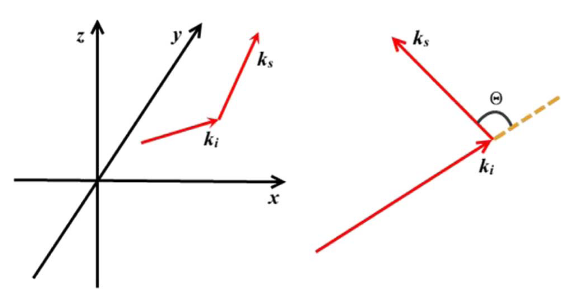
\includegraphics[width=0.62\textwidth]{2frames.png}
  \caption{两种坐标系示意图。左：主坐标系，入射方向 $\bm{k}_i$ 与散射方向 $\bm{k}_s$ 在三维空间中的表示；右：1-2 散射坐标系，散射角 $\Theta$ 为 $\bm{k}_i$ 与 $\bm{k}_s$ 之间的夹角。}
  \label{fig:frames}
\end{figure}

\paragraph{1-2 坐标系（局部散射坐标系）}
在该坐标系下，相矩阵仅依赖于单一变量——散射角 $\Theta$（即入射波方向与散射波方向之间的夹角）。1 极化方向垂直于由入射辐射方向和散射辐射方向共同构成的"散射平面"，2 极化方向平行于散射平面。这种基于物理对称性的简化使得相矩阵可直接表示为 $\overline{\overline{P}}(\Theta)$，适合在蒙特卡洛光线追踪中进行统计计算。

\paragraph{主坐标系（极化参考坐标系）}
主坐标系是地球遥感领域默认的标准极化参考坐标系，水平极化方向严格定义为平行于地球表面（即 $zy$ 平面）。主坐标系下的相矩阵需要由四个几何角度共同描述：入射方向的极角 $\theta_i$ 和方位角 $\varphi_i$，以及散射方向的极角 $\theta_s$ 和方位角 $\varphi_s$，记为 $\overline{\overline{P}}(\theta_s, \varphi_s; \theta_i, \varphi_i)$。

\subsection{坐标系变换}

在蒙特卡洛光线追踪过程中，1-2 坐标系下计算相矩阵更为方便。为便于代入辐射传输方程（使用主坐标系），需通过旋转矩阵将 $\overline{\overline{P}}(\Theta)$ 变换至主坐标系：
\begin{equation}
  \bar{\bar{P}}(\theta_s,\varphi_s;\theta_i,\varphi_i)
  = L(\sigma_2) \cdot \bar{\bar{P}}(\Theta) \cdot L(-\sigma_1),
  \label{eq:pm-transform}
\end{equation}
其中旋转矩阵为
\begin{equation}
  L(\sigma) =
  \begin{pmatrix}
    1 & 0 & 0 & 0 \\
    0 & \cos 2\sigma & \sin 2\sigma & 0 \\
    0 & -\sin 2\sigma & \cos 2\sigma & 0 \\
    0 & 0 & 0 & 1
  \end{pmatrix}.
  \label{eq:rotation-matrix}
\end{equation}
旋转角 $\sigma_1$ 是入射方向的 $\hat{e}_v$ 相对于 1-2 系 $\hat{e}_1$ 方向的旋转角，$\sigma_2$ 是散射方向 1-2 系 $\hat{e}_1$ 相对于主参考系 $\hat{e}_v$ 方向的旋转角。

\subsection{散射系数与相矩阵的关系}

散射系数 $\kappa_s$ 与 1-2 坐标系下相矩阵之间满足
\begin{equation}
  \kappa_s = \pi \int_0^\pi
  \bigl(P_{11}(\Theta)+P_{22}(\Theta)+P_{12}(\Theta)+P_{21}(\Theta)\bigr)
  \sin\Theta\,\mathrm{d}\Theta.
  \label{eq:kappa-s}
\end{equation}
在几何光学限制下，散射效应仅由反射或折射引起，可近似认为 $P_{12}=P_{21}=0$，故式~\eqref{eq:kappa-s} 离散后为
\begin{equation}
  \kappa_s \approx \pi \sum_i
  \bigl(P_{11}(\Theta_i)+P_{22}(\Theta_i)\bigr)
  \sin\Theta_i\,\Delta\Theta_i.
  \label{eq:kappa-s-discrete}
\end{equation}
式~\eqref{eq:kappa-s-discrete} 同时用于对相矩阵统计结果归一化，确保其具有绝对量纲。

\subsection{蒙特卡洛算法实现}

本项目采用蒙特卡洛光线追踪方法计算 $P_{11}(\Theta)$ 和 $P_{22}(\Theta)$，大体思路为
\begin{enumerate}
  \item 在介质内随机取点、随机方向射出光线，\textbf{DDA算法追踪光线}直至碰撞到两相交界或飞出界面。
  \item 假设两相交界理想平坦，可以应用斯涅尔定律和菲涅尔定理来确定散射角度，以及\textbf{散射到这些角度上的强度分量}。
  \item 记录交界处发生的折射和散射，将反射能量 $I_r$ 和折射能量 $I_t$ \textbf{累加到对应角度区间}。
  \item 累计权重通过采用 $\kappa_s$ 公式来归一化相矩阵数值为绝对量纲。
\end{enumerate}
具体步骤如算法~\ref{alg:phase-matrix} 所示。

\begin{algorithm}[H]
\caption{蒙特卡洛相矩阵统计算法}
\label{alg:phase-matrix}
\KwIn{双连续介质体素数组，光线数 $N_\text{ray}$，角度区间数 $N_\text{bin}$，散射系数 $\kappa_s$}
\KwOut{相矩阵分量 $P_{11}(\Theta)$，$P_{22}(\Theta)$}
初始化 $\mathtt{acc\_P11}[N_\text{bin}]\leftarrow 0$，$\mathtt{acc\_P22}[N_\text{bin}]\leftarrow 0$\;
\For{$\mathrm{ray}=1$ \KwTo $N_\text{ray}$}{
  在介质内随机取起始点 $\bm{r}$，随机采样入射方向 $\hat{d}$\;
  \textbf{DDA 算法}：沿 $\hat{d}$ 追踪光线，直至命中两相界面，记录界面坐标及法向量 $\hat{n}$\;
  计算入射余弦 $\cos\theta_i = |\hat{d}\cdot\hat{n}|$，确定折射率 $n_1, n_2$\;
  由菲涅耳公式计算反/折射振幅系数 $R_s,R_p,T_s,T_p$ 及全内反射标志 $\mathtt{is\_tir}$\;
  \Comment{处理反射分支}
  由 $\hat{d}$ 和 $\hat{n}$ 计算反射方向 $\hat{r}$，得散射角 $\Theta_r$\;
  $b_r\leftarrow\lfloor\Theta_r/\pi\times N_\text{bin}\rfloor$\;
  $\mathtt{acc\_P11}[b_r]\mathrel{+}=R_s$；$\mathtt{acc\_P22}[b_r]\mathrel{+}=R_p$\;
  \If{$\neg\,\mathtt{is\_tir}$}{
    \Comment{处理折射分支}
    由斯涅耳定律计算折射方向 $\hat{t}$，得散射角 $\Theta_t$\;
    $b_t\leftarrow\lfloor\Theta_t/\pi\times N_\text{bin}\rfloor$\;
    $\mathtt{acc\_P11}[b_t]\mathrel{+}=T_s$；$\mathtt{acc\_P22}[b_t]\mathrel{+}=T_p$\;
  }
}
\Comment{利用式~\eqref{eq:kappa-s-discrete} 归一化}
$\Delta\Theta\leftarrow\pi/N_\text{bin}$；$\Theta_i\leftarrow(i+0.5)\Delta\Theta$\;
$\mathrm{norm}\leftarrow\pi\sum_i\bigl(\mathtt{acc\_P11}[i]+\mathtt{acc\_P22}[i]\bigr)\sin\Theta_i\Delta\Theta$\;
$\mathrm{scale}\leftarrow\kappa_s/\mathrm{norm}$\;
$P_{11}\leftarrow\mathtt{acc\_P11}\times\mathrm{scale}$；$P_{22}\leftarrow\mathtt{acc\_P22}\times\mathrm{scale}$\;
\Return $P_{11},\,P_{22}$
\end{algorithm}





图~\ref{fig:phase-matrix} 展示了仿真所得的相矩阵 $P_{11}(\Theta)$ 与 $P_{22}(\Theta)$ 的角度分布，可观察到显著的前向散射增强特征。

\begin{figure}[htbp]
  \centering
  \begin{subfigure}[b]{0.7\textwidth}
    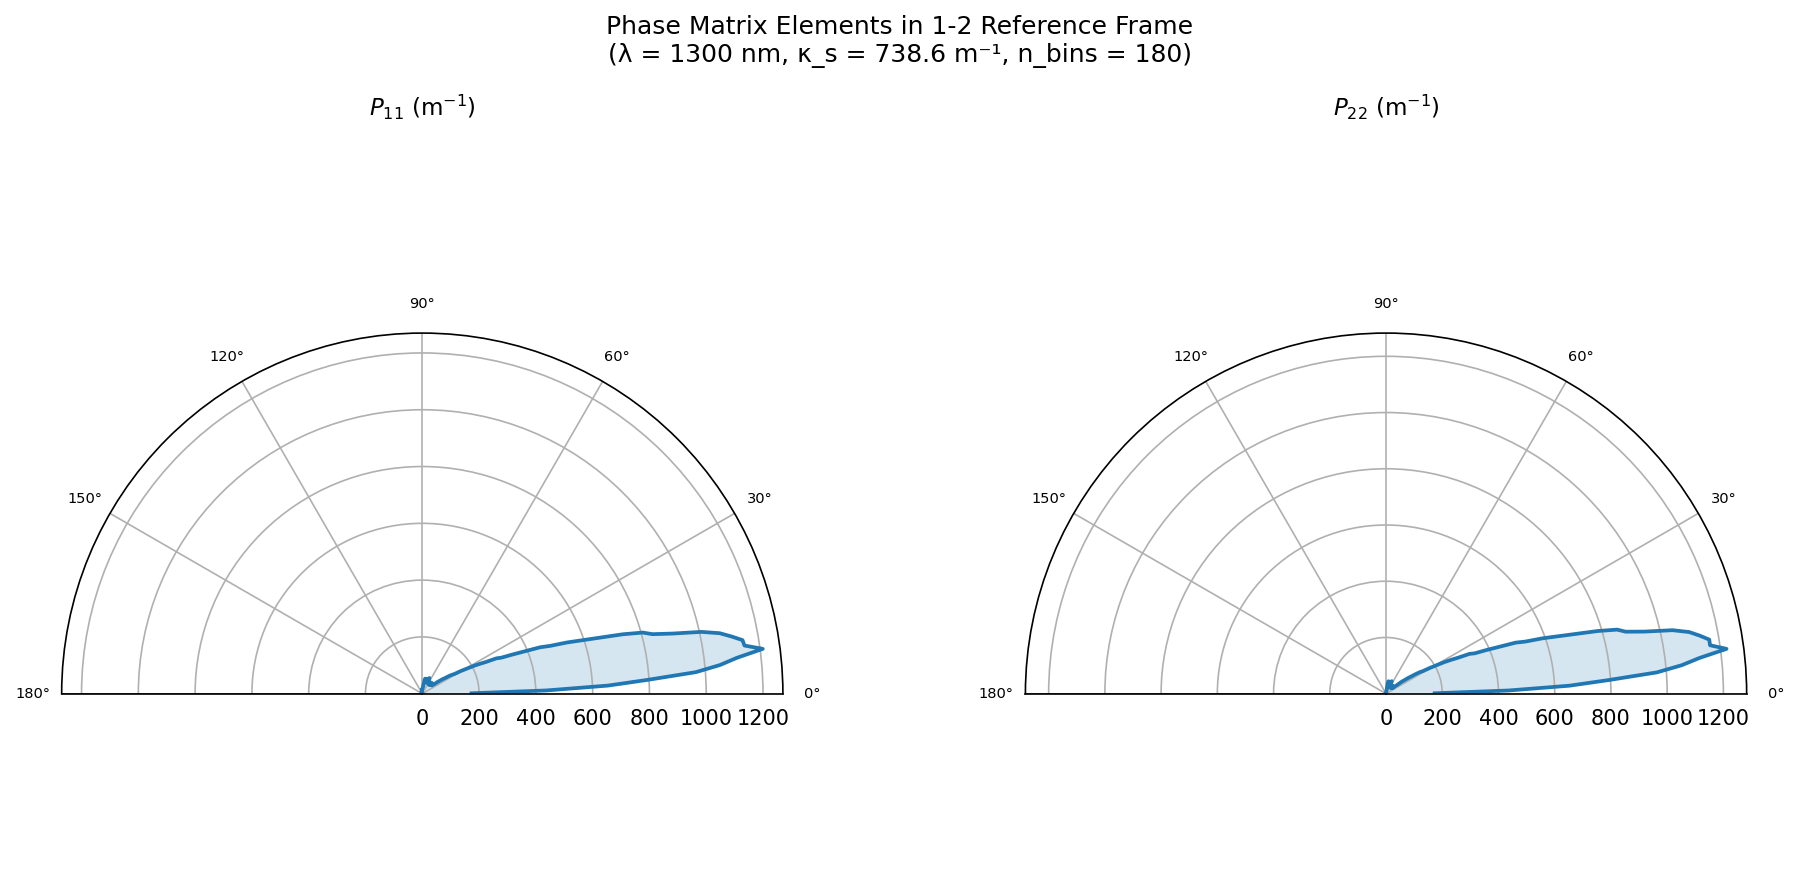
\includegraphics[width=\textwidth]{phase_matrix_polar_ks739.png}
    \caption{极坐标表示}
  \end{subfigure}
  \hfill
  \begin{subfigure}[b]{0.7\textwidth}
    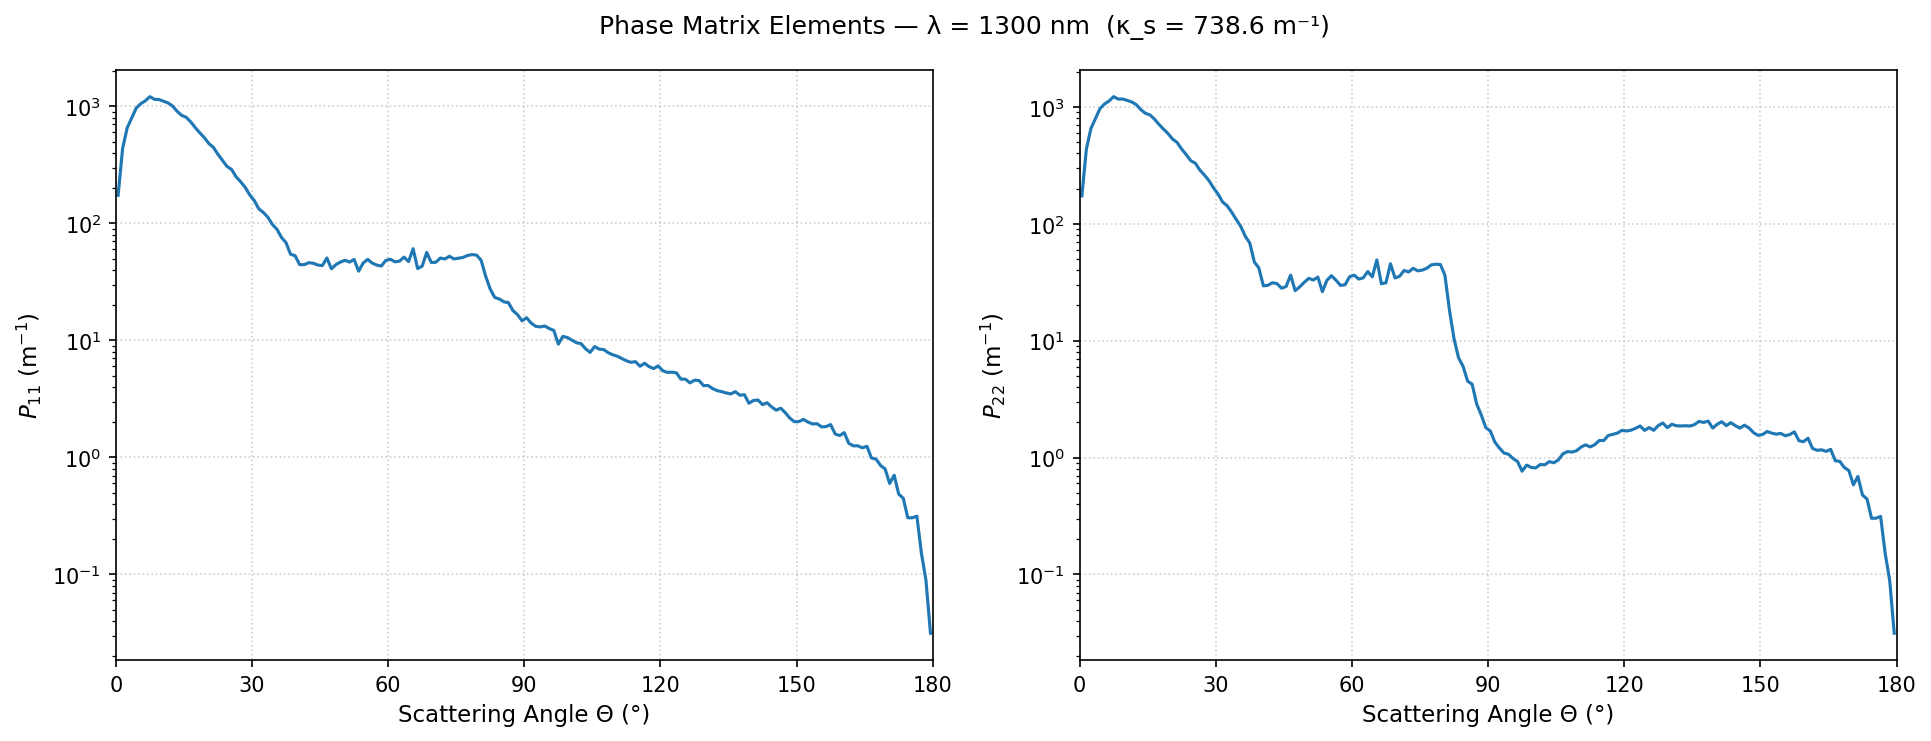
\includegraphics[width=\textwidth]{phase_matrix_cartesian_ks739.png}
    \caption{直角坐标表示}
  \end{subfigure}
  \caption{仿真所得相矩阵元素 $P_{11}(\Theta)$（左侧图）与 $P_{22}(\Theta)$（右侧图）随散射角 $\Theta$ 的分布。}
  \label{fig:phase-matrix}
\end{figure}

% ==================== Section 2：VRT ====================
\section{矢量辐射传输方程求解}
\label{sec:vrt}

\subsection{矢量辐射传输方程}

通过蒙特卡洛光线追踪，已可得到模拟雪介质的微观参量：消光系数 $\kappa_e$、吸收系数 $\kappa_a$、散射系数 $\kappa_s$（满足 $\kappa_e=\kappa_s+\kappa_a$）以及相矩阵 $\overline{\overline{P}}$。将这些参量代入矢量辐射传输方程：
\begin{equation}
  \cos\theta\frac{d\bar{\mathbf{I}}(\theta,\varphi,z)}{dz}
  = -\kappa_e\bar{\mathbf{I}}(\theta,\varphi,z)
  + \int_{-\pi/2}^{\pi/2}\!\sin\theta'\,d\theta'
    \int_0^{2\pi}\!\overline{\overline{\mathbf{P}}}(\theta,\varphi;\theta',\varphi')
    \bar{\mathbf{I}}(\theta',\varphi',z)\,d\varphi'.
  \label{eq:vrt}
\end{equation}

其中 $\bar{\mathbf{I}}=[I_1,I_2,I_3,I_4]^T$ 为斯托克斯矢量，各分量的物理含义为
\begin{equation}
  \bar{\mathbf{I}} =
  \begin{bmatrix} I_1 \\ I_2 \\ I_3 \\ I_4 \end{bmatrix}
  =
  \begin{bmatrix}
    \langle|E_v|^2\rangle \\
    \langle|E_h|^2\rangle \\
    2\,\mathrm{Re}(E_v E_h^*) \\
    2\,\mathrm{Im}(E_v E_h^*)
  \end{bmatrix},
  \label{eq:stokes}
\end{equation}
$I_1$、$I_2$ 分别为垂直极化和水平极化强度分量，$I_3$、$I_4$ 描述两极化分量之间的相位相关性。方程~\eqref{eq:vrt} 各项的物理含义：
\begin{itemize}[leftmargin=2em]
  \item 左端 $\cos\theta\,d\bar{\mathbf{I}}/dz$：辐射强度随雪层深度 $z$ 的变化率，$\cos\theta$ 修正斜入射时光线的有效穿透深度；
  \item 右端第一项 $-\kappa_e\bar{\mathbf{I}}$：消光项，光被吸收或散射至其他方向而损失；
  \item 右端积分项：来自所有其他方向 $(\theta',\varphi')$ 经相矩阵描述的散射"汇入"当前方向的贡献。
\end{itemize}

\subsection{约化项与漫射项分解}

将总辐射场分解为约化项（直射衰减项）与漫射项之和：
\begin{equation}
  \bar{\mathbf{I}} = \bar{\mathbf{I}}^{(R)} + \bar{\mathbf{I}}^{(D)}.
  \label{eq:decomp}
\end{equation}
约化项 $\bar{\mathbf{I}}^{(R)}$ 满足无散射源的衰减方程，其解析解为
\begin{equation}
  \bar{\mathbf{I}}^{(R)}(z)
  = \bar{\mathbf{I}}_0\,\exp\!\left(-\frac{\kappa_e z}{\mu_0}\right),
  \label{eq:reduced}
\end{equation}
其中 $\mu_0=|\cos\theta_0|$ 为入射天顶角余弦。由于可见光和近红外波段空气-雪界面透过率较高（反射率较小），约化项在光学厚介质中迅速衰减，实用中通常忽略。

将式~\eqref{eq:decomp} 代入方程~\eqref{eq:vrt}，展开后利用约化项自身满足消光方程这一条件，两侧约化项对消，可得漫射项方程：
\begin{equation}
  \mu\frac{d\bar{\mathbf{I}}^{(D)}}{dz}
  = -\kappa_e\bar{\mathbf{I}}^{(D)}
  + \int\!\!\int\overline{\overline{\mathbf{P}}}\,\bar{\mathbf{I}}^{(D)}\,d\mu'\,d\varphi'
  + \bar{\mathbf{S}}(\mu,\varphi,z),
  \label{eq:diffuse}
\end{equation}
其中源项 $\bar{\mathbf{S}}$ 来自约化项（直射光）首次被散射产生的漫射光：
\begin{equation}
  \bar{\mathbf{S}}(\mu,\varphi,z)
  = \overline{\overline{\mathbf{P}}}(\mu,\varphi;\mu_0,\varphi_0)\,\bar{\mathbf{I}}_0
    \,\exp\!\left(-\frac{\kappa_e z}{\mu_0}\right).
  \label{eq:source}
\end{equation}
对于非偏振太阳入射，取 $\bar{\mathbf{I}}_0=[0.5,\,0.5,\,0,\,0]^T$。

\subsection{方位角傅里叶展开}

方程~\eqref{eq:diffuse} 包含 $\theta$（天顶角）和 $\varphi$（方位角）两个角度变量，直接求解计算代价极高。利用雪介质各向同性的方位对称性，对漫射光强和相矩阵分别进行傅里叶展开，可将二维问题解耦为一系列一维 ODE：
\begin{equation}
  \bar{\mathbf{I}}^{(D)}(\theta,\varphi,z)
  = \bar{\mathbf{I}}^{(D)}_0(\theta,z)
  + \sum_{m=1}^{M_{\max}}\!\left[
      \bar{\mathbf{I}}^{(D)}_{mc}(\theta,z)\cos m(\varphi-\varphi_0)
    + \bar{\mathbf{I}}^{(D)}_{ms}(\theta,z)\sin m(\varphi-\varphi_0)
  \right],
  \label{eq:fourier-I}
\end{equation}
\begin{equation}
  \overline{\overline{\mathbf{P}}}(\theta,\varphi;\theta',\varphi')
  = \overline{\overline{\mathbf{P}}}_0
  + \sum_{m=1}^{M_{\max}}\!\left[
    \overline{\overline{\mathbf{P}}}_{mc}\cos m(\varphi-\varphi')
  + \overline{\overline{\mathbf{P}}}_{ms}\sin m(\varphi-\varphi')
  \right],
  \label{eq:fourier-P}
\end{equation}
截断阶数取 $M_{\max}=32$。相矩阵傅里叶系数通过 $[0,2\pi]$ 上的 Gauss-Legendre 数值积分计算：
\begin{align}
  \overline{\overline{\mathbf{P}}}_0(\theta;\theta')
  &= \frac{1}{2\pi}\sum_{i=1}^{N}\tilde{w}_i\,
     \overline{\overline{\mathbf{P}}}(\theta,0;\theta',\varphi_i),
  \label{eq:P0} \\
  \overline{\overline{\mathbf{P}}}_{mc}(\theta;\theta')
  &= \frac{1}{\pi}\sum_{i=1}^{N}\tilde{w}_i\,
     \overline{\overline{\mathbf{P}}}(\theta,0;\theta',\varphi_i)\cos(m\varphi_i),
  \label{eq:Pmc} \\
  \overline{\overline{\mathbf{P}}}_{ms}(\theta;\theta')
  &= \frac{1}{\pi}\sum_{i=1}^{N}\tilde{w}_i\,
     \overline{\overline{\mathbf{P}}}(\theta,0;\theta',\varphi_i)\sin(m\varphi_i).
  \label{eq:Pms}
\end{align}
其中 $\varphi_i=\pi(x_i+1)$ 为第 $N$ 阶 Legendre 多项式零点 $x_i\in[-1,1]$ 经线性变换后在 $[0,2\pi]$ 上的积分节点，$\tilde{w}_i=\pi w_i$ 为对应权重。

\subsection{离散坐标法与 ODE 方程组构建}

对每个傅里叶模态，令 $\mu=\cos\theta$，取 $J$ 个 Gauss-Legendre 节点 $\{\mu_j, w_j\}$，将天顶角积分离散化。以第 $m$ 阶为例，方程离散为
\begin{equation}
  \mu_j\frac{d\bar{\mathbf{I}}_m(\mu_j,z)}{dz}
  = -\kappa_e\bar{\mathbf{I}}_m(\mu_j,z)
  + \sum_{k=1}^{J}w_k\,\overline{\overline{\mathbf{P}}}_m(\mu_j;\mu_k)\,\bar{\mathbf{I}}_m(\mu_k,z)
  + \overline{\overline{\mathbf{P}}}_m(\mu_j;\mu_0)\cdot\bar{\mathbf{I}}_0\,e^{-\kappa_e z/\mu_0}.
  \label{eq:discrete-vrt}
\end{equation}
将所有离散方向合并为向量 $\mathbf{I}(z)\in\mathbb{R}^{4J}$，方程~\eqref{eq:discrete-vrt} 化为矩阵 ODE 标准形式：
\begin{equation}
  \frac{d\mathbf{I}(z)}{dz}
  = \mathbf{B}\,\mathbf{I}(z) + \mathbf{F}\,e^{-\kappa_e z/\mu_0},
  \label{eq:ode}
\end{equation}
其中
\begin{equation}
  \mathbf{B} = \mathbf{M}^{-1}\!\left(-\kappa_e\mathbf{E}+\mathbf{W}\mathbf{P}\right),
  \qquad
  \mathbf{F} = \mathbf{M}^{-1}\mathbf{Q}.
  \label{eq:BF}
\end{equation}
各矩阵的定义如下：
\begin{itemize}[leftmargin=2em]
  \item $\mathbf{M}=\mathrm{diag}(\mu_1,\mu_1,\mu_1,\mu_1,\,\mu_2,\ldots)$：$4J\times4J$ 天顶角余弦对角矩阵；
  \item $\mathbf{W}=\mathrm{diag}(w_1,w_1,w_1,w_1,\,w_2,\ldots)$：Gauss-Legendre 权重对角矩阵；
  \item $\mathbf{P}$：$4J\times4J$ 分块相矩阵，$[\mathbf{P}]_{jk}=\overline{\overline{\mathbf{P}}}_m(\mu_j;\mu_k)$；
  \item $\mathbf{Q}$：$4J\times1$ 源向量，$[\mathbf{Q}]_j=\overline{\overline{\mathbf{P}}}_m(\mu_j;\mu_0)\cdot\bar{\mathbf{I}}_0$。
\end{itemize}

\subsection{特征值法求解与边界条件}

\subsubsection{特解}
假设特解形式为 $\mathbf{I}^{(p)}(z)=\mathbf{C}\,e^{-\kappa_e z/\mu_0}$，代入方程~\eqref{eq:ode} 可得
\begin{equation}
  \mathbf{C} = -\!\left(\mathbf{B}+\frac{\kappa_e}{\mu_0}\mathbf{E}\right)^{-1}\!\mathbf{F}.
  \label{eq:particular}
\end{equation}
当矩阵奇异时，用最小二乘法代替精确求逆。

\subsubsection{齐次解}
方程~\eqref{eq:ode} 的齐次解为
\begin{equation}
  \mathbf{I}^{(h)}(z) = \sum_{l=1}^{4J}c_l\,\mathbf{v}_l\,e^{\lambda_l z},
  \label{eq:homogeneous}
\end{equation}
其中 $\lambda_l$ 和 $\mathbf{v}_l$ 为 $\mathbf{B}$ 的特征值和特征向量，满足 $\mathbf{B}\mathbf{v}_l=\lambda_l\mathbf{v}_l$。特征值正好对应不同的光传播衰减模式：
\begin{equation}
  \underbrace{\lambda_1^+>\lambda_2^+>\cdots>0}_{\text{正特征值：向下传播增长模}}
  \quad>\quad
  \underbrace{0>\cdots>\lambda_1^->...>\lambda_{2J}^-}_{\text{负特征值：向上传播衰减模}}.
\end{equation}

\subsubsection{边界条件}

下面利用两个物理边界条件确定通解系数。

\textbf{条件 1（光学半无限条件）：} 雪层光学厚度足够大，当 $z\to\infty$ 时光强有界。因此所有对应正特征值的模态系数均为零：
\begin{equation}
  c_l^+=0, \quad l=1,2,\ldots,2J.
  \label{eq:bc1}
\end{equation}
通解化简为
\begin{equation}
  \mathbf{I}(z)
  = \sum_{l=1}^{2J}c_l^-\,\mathbf{v}_l^-\,e^{\lambda_l^- z}
  + \mathbf{C}\,e^{-\kappa_e z/\mu_0}.
  \label{eq:general-solution}
\end{equation}
为便于理解，可写为
\begin{equation}
    \mathbf{I}(z) = \boxed{ c^-_1\begin{pmatrix}
 v_{1,1}  \\
  \vdots \\
  v_{1,4J} \\
  
\end{pmatrix}+c^-_2\begin{pmatrix}
 v_{2,1}  \\
   \vdots\\
  v_{2,4J}
\end{pmatrix}+\cdots+c^-_{2J}\begin{pmatrix}
  v_{2J,1} \\
  \vdots \\
  v_{2J,4J}
\end{pmatrix}}+ \mathbf{C}\cdot e^{-\kappa_e z/\mu_0}
\end{equation}

\textbf{条件 2（表面无漫射入射）：} 在雪表面 $z=0$，无外来向下传播的漫射辐射（认为射入雪层的光在底部消散，不会反射后重新向下传播）：
\begin{equation}
  \mathbf{I}^{(D)}(\mu_j,z=0) = \mathbf{0},
  \quad\text{对所有 } \mu_j<0 \text{（向下方向）}.
  \label{eq:bc2}
\end{equation}
由此得线性方程组
\begin{equation}
  \mathbf{V}^{(\downarrow)}\,\mathbf{c} = -\mathbf{C}^{(\downarrow)},
  \label{eq:linear-system}
\end{equation}
其中 $\mathbf{V}^{(\downarrow)}$ 为所有负特征向量在向下分量方向的子矩阵，$\mathbf{C}^{(\downarrow)}$ 为特解在向下分量方向的子向量。用最小二乘法求解系数向量 $\mathbf{c}$。

\subsubsection{雪面向上漫射辐射}

确定系数后，雪表面 $z=0$ 处向上传播的漫射辐射为
\begin{equation}
  \mathbf{I}^{(\uparrow)}(0)
  = \mathbf{V}^{(\uparrow)}\,\mathbf{c} + \mathbf{C}^{(\uparrow)}.
  \label{eq:upward}
\end{equation}
将所有傅里叶模态叠加，得到完整出射辐射场：
\begin{equation}
  \bar{\mathbf{I}}^{(D)}(\mu_s,\varphi_s,0)
  = \bar{\mathbf{I}}^{(D)}_0(\mu_s,0)
  + \sum_{m=1}^{M_{\max}}\!\left[
    \bar{\mathbf{I}}^{(D)}_{mc}(\mu_s,0)\cos m(\varphi_s-\varphi_0)
  + \bar{\mathbf{I}}^{(D)}_{ms}(\mu_s,0)\sin m(\varphi_s-\varphi_0)
  \right].
  \label{eq:reconstruct}
\end{equation}

\subsection{算法流程与代码实现}

算法~\ref{alg:vrt} 给出矢量辐射传输方程的完整求解流程。

\begin{algorithm}[htbp]
\caption{矢量辐射传输方程特征值法求解}
\label{alg:vrt}
\KwIn{$\kappa_e$，$P_{11}(\Theta)$，$P_{22}(\Theta)$，太阳天顶角 $\theta_0$，方位角 $\varphi_0$，入射 Stokes 矢量 $\bar{\mathbf{I}}_0$，离散流数 $J$，Fourier 截断阶数 $M_{\max}$}
\KwOut{出射 Stokes 矢量场 $\bar{\mathbf{I}}^{(D)}(\mu_s,\varphi_s,0)$}
$\mu_0\leftarrow-|\cos\theta_0|$ \Comment*[r]{内部约定：入射方向对应负 $\mu$}
采样 Gauss-Legendre 节点 $\{\mu_j,w_j\}_{j=1}^{J}$（天顶角离散化）\;
采样 Gauss-Legendre 节点 $\{\varphi_i,\tilde{w}_i\}_{i=1}^{N}$（方位角积分节点）\;
\For{$m=0$ \KwTo $M_{\max}$}{
  \For{所有 $(\mu_j,\mu_k)$ 节点对}{
    由式~\eqref{eq:pm-transform} 计算 $\overline{\overline{\mathbf{P}}}(\mu_j,0;\mu_k,\varphi_i)$\;
    由式~\eqref{eq:P0}--\eqref{eq:Pms} 计算 Fourier 系数 $\overline{\overline{\mathbf{P}}}_m(\mu_j;\mu_k)$\;
  }
  由式~\eqref{eq:BF} 构建 ODE 矩阵 $\mathbf{B}$ 和源向量 $\mathbf{F}$\;
  由式~\eqref{eq:particular} 计算特解系数矩阵 $\mathbf{C}$\;
  对 $\mathbf{B}$ 进行特征值分解，筛选负特征值模态（式~\eqref{eq:bc1}）\;
  由式~\eqref{eq:linear-system} 求解边界条件线性方程组，得系数向量 $\mathbf{c}$\;
  由式~\eqref{eq:upward} 计算第 $m$ 阶模态的向上辐射 $\mathbf{I}_m^{(\uparrow)}(0)$\;
}
由式~\eqref{eq:reconstruct} 叠加所有 Fourier 模态，重建完整辐射场\;
\Return $\bar{\mathbf{I}}^{(D)}(\mu_s,\varphi_s,0)$
\end{algorithm}


% ==================== Section 3：反射率参数 ====================
\section{雪面反射特性计算}
\label{sec:reflectance}

利用式~\eqref{eq:reconstruct} 得到的雪面向上漫射辐射场，可进一步计算四类宏观光学参数。

\subsection{双向反射分布函数（BRDF）}

\textbf{物理含义：}
BRDF（Bidirectional Reflectance Distribution Function，双向反射分布函数）是同时依赖入射方向 $(\theta_i,\varphi_i)$ 和出射方向 $(\theta_s,\varphi_s)$ 的四维函数，完整刻画了表面反射的各向异性结构。它是反射辐射亮度对入射辐照度的微分比，单位为 $\mathrm{sr}^{-1}$。与简单无量纲反射率不同，BRDF 是描述辐射场方向分布的场量。雪面反射具有显著的非朗伯特征：前向散射方向反射最强，前后向最大差异可达 3--5 倍（依波长而异），忽略 BRDF 效应将引起积雪参数反演的系统误差。

\textbf{数学定义：}
\begin{equation}
  \rho(\theta_s,\varphi_s,\theta_0)
  = \frac{I_1^{(D)}(\mu_s,\varphi_s,0)+I_2^{(D)}(\mu_s,\varphi_s,0)}{\mu_0}.
  \label{eq:brdf}
\end{equation}

\subsection{半球反照率（Albedo）}

\textbf{物理含义：}
反照率是地表向整个上半球方向反射的辐射通量与到达地表入射辐射通量之比，无量纲，是 BRDF 对出射半球方向的积分量，也是地表能量收支计算的核心参数。新鲜干雪宽带反照率高达 0.85--0.95，旧雪、湿雪或含杂质雪可低至 0.40 以下，对气候能量平衡（冰雪-反照率反馈机制）影响巨大。卫星只能观测特定方向的辐亮度，必须通过 BRDF 模型将方向反射转换为半球反照率，否则存在显著的方向误差。

\textbf{数学定义：}
\begin{equation}
  \alpha(\theta_0)
  = \int_0^{2\pi}\!\int_0^{\pi/2}\!
    \rho(\theta_s,\varphi_s,\theta_0)\,\cos\theta_s\sin\theta_s\,d\theta_s\,d\varphi_s.
  \label{eq:albedo}
\end{equation}
项目同时支持基于 $m=0$ 模态的快速半解析积分和基于离散 BRDF 网格的数值积分两种方式。

\subsection{各向异性反射因子（ARF）}

\textbf{物理含义：}
ARF（Anisotropic Reflectance Factor，各向异性反射因子）是描述地表偏离朗伯（各向同性）反射程度的无量纲归一化因子。其核心思想是：将真实表面与具有相同总反照率的假想朗伯体进行比较——$\mathrm{ARF}>1$ 说明该方向反射比等效朗伯体更强，$\mathrm{ARF}=1$（所有方向）对应完美朗伯体。雪面和冰面的 ARF 分布范围可达 0.56--1.72（随波段和太阳高度角变化），常用于卫星观测的角度归一化校正以及极区能量平衡的辐射通量方向校正。

\textbf{数学定义：}
\begin{equation}
  \mathrm{ARF}(\theta_s,\varphi_s,\theta_0)
  = \frac{\pi\cdot\rho(\theta_s,\varphi_s,\theta_0)}{\alpha(\theta_0)}.
  \label{eq:arf}
\end{equation}
可以验证，对 $\mathrm{ARF}$ 在出射半球加权积分恢复为 $\pi$，满足能量归一化约束；$\mathrm{ARF}$ 是 BRDF 的归一化形式，消除了反照率绝对值的影响，纯粹表征方向分布的形状。

\subsection{极化双向反射分布函数（极化 BRDF）}

\textbf{物理含义：}
极化 BRDF（Polarized BRDF，pBRDF）是 BRDF 的极化扩展形式，不仅包含反射强度，还包含偏振度（Degree of Polarization，DoP）、偏振方向（Angle of Polarization，AoP）等极化状态信息。雪面极化的主要物理机制来自：\textit{菲涅耳反射极化}（$s/p$ 分量反射率差异产生线偏振）和\textit{单次散射极化}（冰晶粒子散射的固有极化特征），多次散射则使偏振度下降。pBRDF 对雪粒径的灵敏度远高于标量 BRDF，可用于比表面积（SSA）反演，以及区分新雪、粒雪、冻结壳等不同变质状态。

\textbf{数学定义：}
\begin{equation}
  \rho^{\mathrm{pol}}(\theta_s,\varphi_s,\theta_0)
  = \frac{\sqrt{(I_1^{(D)}-I_2^{(D)})^2+(I_3^{(D)})^2+(I_4^{(D)})^2}}{\mu_0}.
  \label{eq:pol-brdf}
\end{equation}
分子为出射 Stokes 矢量的极化辐射亮度强度，分母 $\mu_0$ 的选取与式~\eqref{eq:brdf} 保持一致。

\subsection{数值结果}

反射率相关参数导出核心代码如下：

\begin{lstlisting}[caption={BRDF/极化BRDF/Albedo/ARF 导出核心（radiative\_transfer\_solver.py）},label={lst:reflectance-export}]
for i, theta_deg in enumerate(theta_samples_deg):
    mu_s = float(np.cos(np.deg2rad(theta_deg)))
    if mu_s <= 0.0:
        continue
    for j, phi_deg in enumerate(phi_samples_deg):
        phi_rad = float(np.deg2rad(phi_deg))
        stokes = self.evaluate_surface_stokes(
            mu_s=mu_s, phi_s=phi_rad, solution=solution)
        brdf_val = (stokes[0] + stokes[1]) / solution.mu0
        pol_val  = np.sqrt((stokes[0] - stokes[1])**2
                           + stokes[2]**2 + stokes[3]**2) / solution.mu0
        brdf[i, j]     = max(float(brdf_val), 0.0)
        pol_brdf[i, j] = max(float(pol_val),  0.0)

albedo_from_grid  = self.integrate_albedo_from_brdf_grid(
    theta_samples_deg=theta_samples_deg,
    phi_samples_deg=phi_samples_deg,
    brdf=brdf)
albedo_from_mode0 = self.compute_albedo(solution=solution)
albedo = albedo_from_grid if albedo_from_grid > 0.0 else albedo_from_mode0
arf    = self.compute_arf_from_brdf(brdf=brdf, albedo=albedo)
\end{lstlisting}

图~\ref{fig:reflectance} 展示了仿真所得的 BRDF、极化 BRDF、反照率和 ARF 空间分布，图~\ref{fig:albedo-sza} 给出了半球反照率随太阳天顶角的变化规律。

\begin{figure}[htbp]
  \centering
  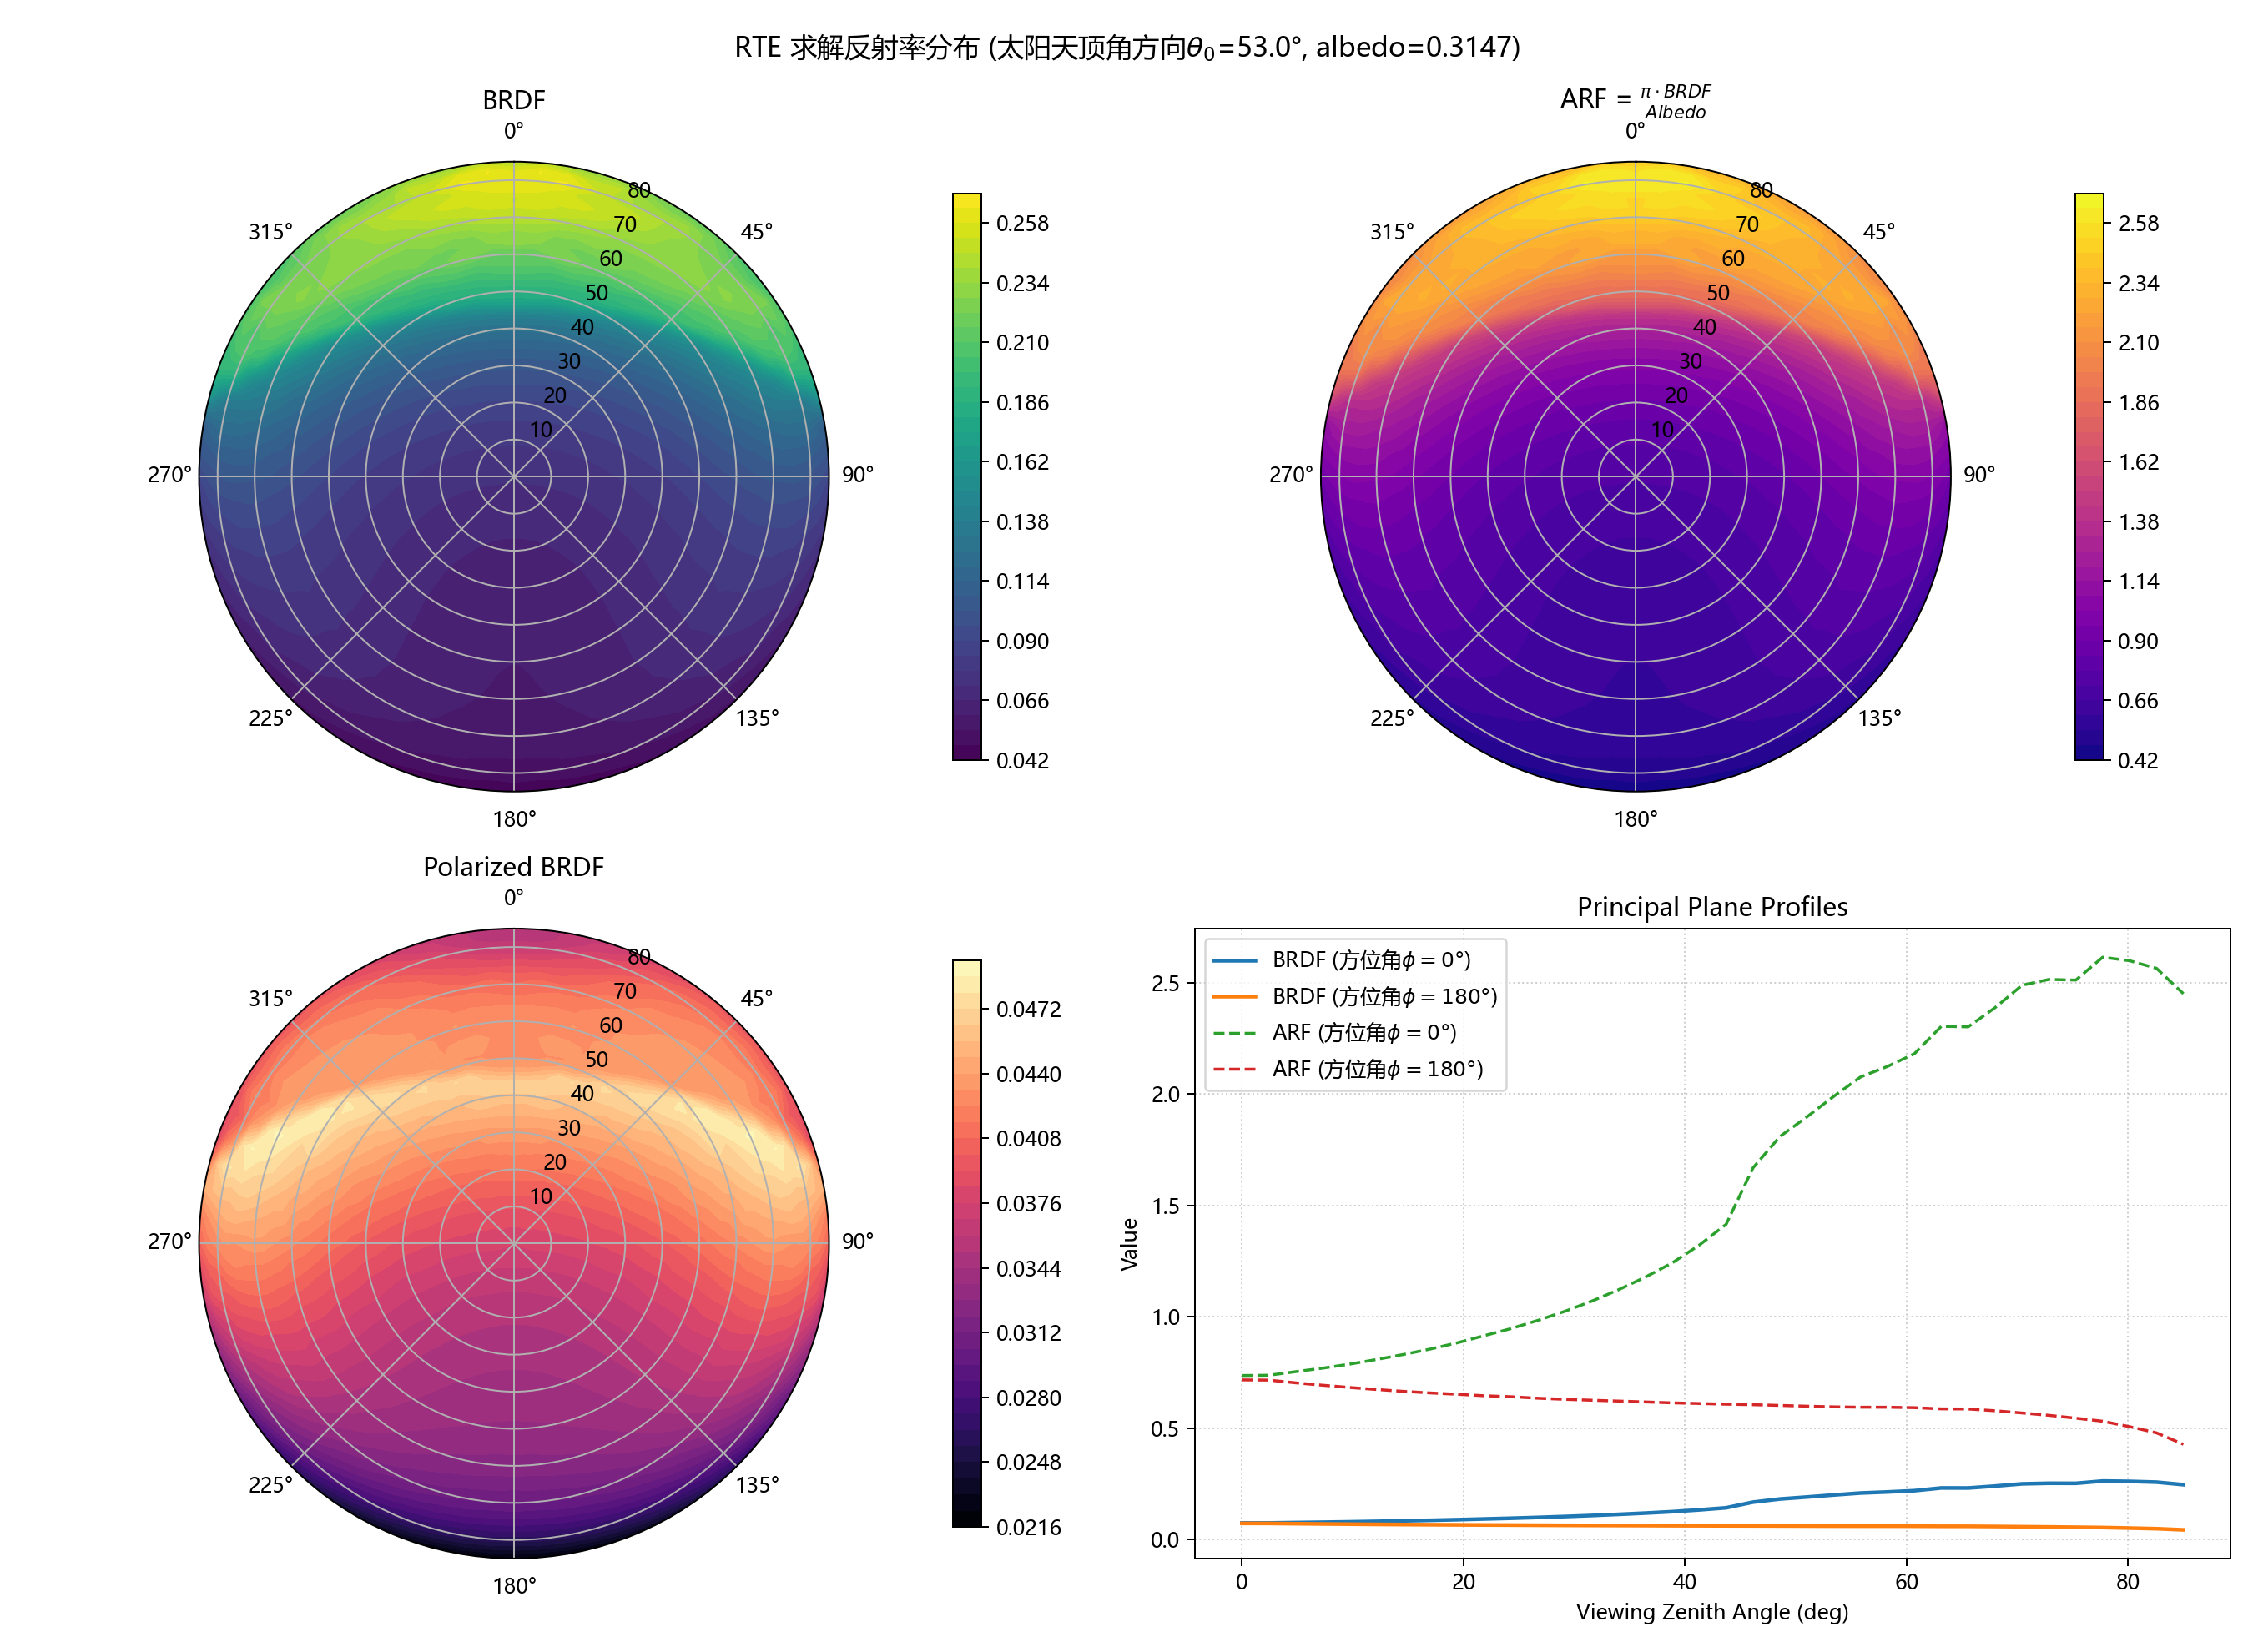
\includegraphics[width=0.9\textwidth]{rte_reflectance.png}
  \caption{仿真所得雪面反射特性：BRDF（式~\eqref{eq:brdf}）、极化 BRDF（式~\eqref{eq:pol-brdf}）、反照率（式~\eqref{eq:albedo}）和 ARF（式~\eqref{eq:arf}）的角度分布。}
  \label{fig:reflectance}
\end{figure}

\begin{figure}[htbp]
  \centering
  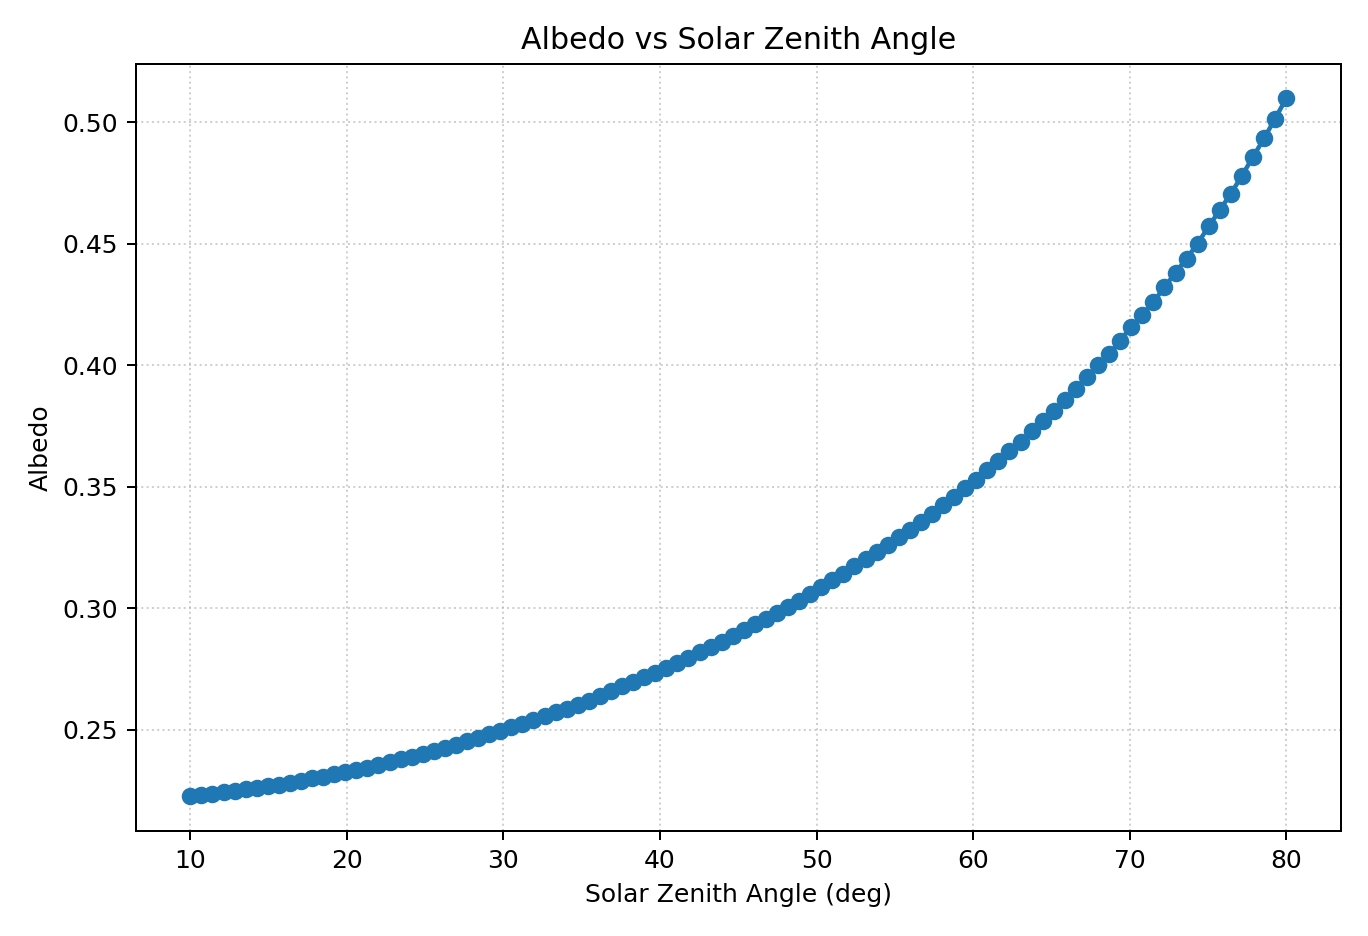
\includegraphics[width=0.62\textwidth]{rte_albedo_vs_sza.png}
  \caption{雪面半球反照率 $\alpha(\theta_0)$（式~\eqref{eq:albedo}）随太阳天顶角 $\theta_0$ 的变化。}
  \label{fig:albedo-sza}
\end{figure}

% ==================== Section 4：与现实雪层的联系 ====================
\section{与现实雪层参数的联系}


在构建模拟雪层介质时，双连续介质模型使用三个微观参量描述雪层结构：
\begin{itemize}[leftmargin=2em]
  \item 平均波数 $\langle\varsigma\rangle$（控制介质的特征空间尺度）；
  \item 粒径分布参数 $b$（控制波数谱的形状）；
  \item 冰体积分数 $f_v$（控制雪层密度）。
\end{itemize}
而实际测量和遥感应用中更常用的雪层描述参量为：
\begin{itemize}[leftmargin=2em]
  \item 雪层密度 $\rho_{\mathrm{snow}}$；
  \item 比表面积（Surface Specific Area）$\mathrm{SSA}$；
  \item 等效晶粒半径 $R_e$。
\end{itemize}

两组参量之间由以下关系联系：
\begin{equation}
  f_v = \frac{\rho_{\mathrm{snow}}}{\rho_{\mathrm{ice}}},
  \label{eq:fv}
\end{equation}
\begin{equation}
  \mathrm{SSA}
  = \frac{2\langle\varsigma\rangle\,e^{-\!\left(\mathrm{erfinv}(1-2f_v)\right)^2}}
         {0.918\pi\sqrt{3}\,f_v}
    \sqrt{\frac{b+2}{b+1}},
  \label{eq:ssa}
\end{equation}
\begin{equation}
  R_e = \frac{3}{0.918\cdot\mathrm{SSA}}.
  \label{eq:re}
\end{equation}
项目在 \texttt{basic\_utils.py} 中的 \texttt{convert\_ssa\_re\_to\_medium\_params} 接口实现了上述转换。这使得模型既可从"生成参数"驱动，也可从"观测参数"反推，便于与实测雪样参数对齐，是连接微观仿真模型与宏观遥感观测的关键桥梁。

% ==================== Section 5：总结与展望 ====================
\section{整体项目总结与展望}

\subsection{完整计算链路}

项目已形成从现实雪层参数到宏观光学散射特性的完整计算链路：
\[
  \text{现实参数}
  \xrightarrow{(1)}
  \text{双连续介质}
  \xrightarrow{(2)}
  \kappa_e
  \xrightarrow{(3)}
  \kappa_a
  \xrightarrow{(4)}
  \overline{\overline{P}}
  \xrightarrow{(5)}
  \text{VRT求解}
  \xrightarrow{(6)}
  \text{BRDF/Albedo/ARF}
\]
核心模块如下：
\begin{enumerate}[leftmargin=2em]
  \item \texttt{bicontinuous\_medium.py}：高斯随机场与二值化雪介质生成、缓存复用；
  \item \texttt{extinction\_calculator.py}：DDA + Monte Carlo 计算投影消光截面并拟合 $\kappa_e$；
  \item \texttt{absorption\_calculator.py}：界面反/折射路径追踪与吸收系数拟合；
  \item \texttt{phase\_matrix\_calculator.py}：$P_{11}/P_{22}$ 角散射统计（见第~\ref{sec:pm} 节）；
  \item \texttt{radiative\_transfer\_solver.py}：Fourier 展开 + 离散坐标 + 特征值法求解 VRT（见第~\ref{sec:vrt} 节）。
\end{enumerate}

\subsection{存在问题}

\begin{enumerate}[leftmargin=2em]
  \item \textbf{简化偏振耦合}：当前实现使用 $\mathrm{diag}(P_{11},P_{22},0,0)$，忽略了完整 $4\times4$ Mueller 矩阵中的跨 Stokes 分量耦合项（$P_{13},P_{14}$ 等），对具有强偏振特征的入射光（如激光）可能不适用。
  \item \textbf{单层平面边界}：目前假设半无限均匀雪层，未覆盖多层雪层结构、底层边界耦合及薄雪层情形。
  \item \textbf{波段局限}：计算假设和近似主要适用于可见光及近红外波段（几何光学近似成立），对短波长或微波波段不适用。
\end{enumerate}

\subsection{未来方向}

\begin{enumerate}[leftmargin=2em]
  \item 扩展完整 $4\times4$ Mueller 相矩阵，实现全偏振耦合，支持偏振光（如激光）入射仿真；
  \item 不同波长的光线对应的冰折射率不同，可尝试引入波长依赖的折射率模型，模拟多波段反射特性；
  \item 增加多层雪层、底边界及大气-雪耦合边界条件，处理有限厚度雪层场景；
  \item 对接实测 BRDF/ARF 数据集进行系统误差校准与模型验证。
\end{enumerate}

\end{document}
